%%%%%%%%%%%%%%%%%%%%%%%%%%%%%%%%%%%%%%
\newcommand{\varLocation}[2]{\varSymbol{loc}{#1}{#2}}
\newcommand{\setLocation}[2]{\setSymbol{LOC}{#1}{#2}}
\newcommand{\formalVarLocation}[2]{(x,y)}
\newcommand{\formalSetLocation}[2]{(\setRealNumbers{}{} \times \setRealNumbers{}{})}

\newcommand{\functionDeployment}[2]{\functionSignature{conf}{\setAgents{}{}}}
\newcommand{\formalDeployment}[2]{\functionFormal{conf}{\setAgents{}{}}{(\setRealNumbers{}{} \times \setRealNumbers{}{})}}
\newcommand{\functionTaskArc}[2]{\functionSignature{arc}{\varAtomicTask{}{}}}
\newcommand{\formalTaskArc}[2]{\functionFormal{arc}{\setAtomicTask{}{}}{\powerSetAgents{}{}}}
\newcommand{\functionTaskDemandPoint}[2]{\functionSignature{dp}{\varAtomicTask{}{}}}
\newcommand{\formalTaskDemandPoint}[2]{\functionFormal{dp}{\setAtomicTask{}{}}{(\setRealNumbersNonNegative{}{} \times \setRealNumbersNonNegative)}}
\newcommand{\varActiveAgent}[2]{\varAgent{#1}{\oplus}}
\newcommand{\varInactiveAgent}[2]{\varAgent{#1}{\ominus}}
\newcommand{\varSensingAgent}[2]{\varAgent{#1}{\ast}}
\newcommand{\varSinkAgent}[2]{\varAgent{#1}{\Delta}}

\newcommand{\varEnergy}[2]{\varSymbol{e}{#1}{#2}}
\newcommand{\setEnergy}[2]{\setSymbol{E}{#1}{#2}}
%%%%%%%%%%%%%%%%%%%%%%%%%%%%%%%%%%%%

%%%%%%%%%%%%%%%%%%%%%%%%%%%%%%%%%%%%%%

\todo[inline]{PROBLEM - SYSTEM}

\begin{figure}
\centering 
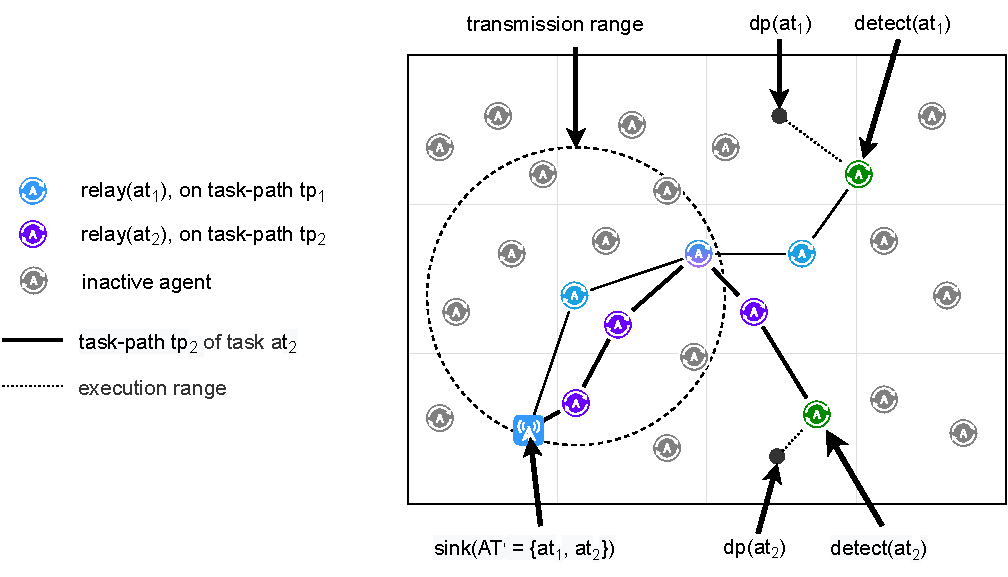
\includegraphics[width=0.9\linewidth]{grid_concept}
\caption[WSN deployment terminology]{WSN deployment terminology}
\label{fig:gridconcept}
\end{figure}

\subsubsection*{Deployment configuration}
Given a geographical area to monitor, we can overlay a two dimensional grid of real numbers, allowing us to associate a deployed set of nodes, or agents, $\setAgents{}{}$, with a corresponding \textit{location}, $\varLocation{}{} = \formalVarLocation{}{} \in \formalSetLocation{}{}$. on the grid. This describes the \textit{deployment configuration} of those agents, a mapping $\formalDeployment{}{}$.


\begin{definition}[Composite task]
	A \textit{composite task}, is composed of $N$ atomic tasks $\varCompositeTask{}{} = \lbrace \varAtomicTask{i}{} \rbrace_{i=0}^N$ where for each of the $i\in N$ grid blocks of the systems geographical grid area.
\end{definition}

\begin{definition}[Atomic task]
	An \textit{atomic task} $\varAtomicTask{\varLocation{}{}}{}$ is a task to take a measurement at a target location $\varLocation{}{}$. The task can be completed by any agent, no matter its distance from the target point.
\end{definition}

\begin{definition}[Demand point]
	A \textit{demand point} is a specific location associated with an atomic task $\functionTaskDemandPoint{}{}$.
\end{definition}


\subsubsection*{Node roles and task arcs}
We can distinguish agents by the role they play in a given atomic task. A \textit{sink node} of an atomic task $\varAtomicTask{}{}$ is the agent that first receives the corresponding composite task, and will broadcast the results. A \textit{sensing node}, $\varSinkAgent{}{}$, is the agent that executes the atomic task and so performs the sensor measurement. An \textit{active node}, $\varActiveAgent{}{}$, is an agent that participates in sub-allocating, or routing, that task, but is neither a sink agent nor a sensing agent. An \textit{inactive agent} does not participate in the task in any way.

With these roles in mind, we can now define the \textit{task arc} as a mapping of atomic tasks to ordered sets of agents $\formalTaskArc{}{}$ that each atomic task $\varAtomicTask{}{}$ is sub-allocated to. The first agent is the agent that has received the initial composite task, and the last agent is the agent that executes the atomic task such that, 
$\functionTaskArc{}{} = \lbrace \varSinkAgent{}{}, \varActiveAgent{i}{}, \varSensingAgent{}{} \rbrace_{i=1}^{n}$. Where there are $n$ active agents sub-allocating the task between the sink and sensing agents.



